\documentclass[a4paper,table,xcdraw]{article}
\usepackage[utf8]{inputenc}
\usepackage[spanish]{babel}
\usepackage{float}
\usepackage{pdfpages}
\usepackage{graphicx}
\usepackage{fancyhdr}
\usepackage{lastpage}
\usepackage{minted}
\usepackage{color,soul}
\usepackage{geometry}
\usepackage{url}
\usepackage{comment}
\usepackage{listings}
\usepackage{courier}
\usepackage{caption}
\usepackage{hyperref}
\usepackage{longtable}

\lstset{
tabsize=4,
numbers=left,
stepnumber=2,
keywordstyle=\color{blue},
frame=single,
basicstyle=\fontsize{11}{13}\ttfamily\footnotesize,
showspaces=false,
showstringspaces=false,
captionpos=b,
breaklines=true
}

\geometry{
 a4paper,
 total={210mm,297mm},
 left=22mm,
 right=19.1mm,
 top=25.4mm,
 bottom=25.4mm,
}

\begin{document}

%%%%%%%%%%%%%%%%%%%%%%%%%%%%%%%%%%%%%%%%%
% University Assignment Title Page 
% LaTeX Template
% Version 1.0 (27/12/12)
%
% This template has been downloaded from:
% http://www.LaTeXTemplates.com
%
% Original author:
% WikiBooks (http://en.wikibooks.org/wiki/LaTeX/Title_Creation)
%
% License:
% CC BY-NC-SA 3.0 (http://creativecommons.org/licenses/by-nc-sa/3.0/)
% 
% Instructions for using this template:
% This title page is capable of being compiled as is. This is not useful for 
% including it in another document. To do this, you have two options: 
%
% 1) Copy/paste everything between \begin{document} and \end{document} 
% starting at \begin{titlepage} and paste this into another LaTeX file where you 
% want your title page.
% OR
% 2) Remove everything outside the \begin{titlepage} and \end{titlepage} and 
% move this file to the same directory as the LaTeX file you wish to add it to. 
% Then add \input{./title_page_1.tex} to your LaTeX file where you want your
% title page.
%
%%%%%%%%%%%%%%%%%%%%%%%%%%%%%%%%%%%%%%%%%

%----------------------------------------------------------------------------------------
%	PACKAGES AND OTHER DOCUMENT CONFIGURATIONS
%----------------------------------------------------------------------------------------

\begin{titlepage}

\newcommand{\HRule}{\rule{\linewidth}{0.5mm}} % Defines a new command for the horizontal lines, change thickness here

\center % Center everything on the page
 
%----------------------------------------------------------------------------------------
%	HEADING SECTIONS
%----------------------------------------------------------------------------------------

\textsc{\LARGE Universidad de Buenos Aires}\\[0.5cm] % Name of your university/college
\textsc{\Large Facultad de Ingeniería}\\[1.5cm] % Major heading such as course name
\textsc{\large 75.67 – Sist. Autom. de Diag. y Detec. de Fallas I}\\[0.5cm] % Minor heading such as course title

%----------------------------------------------------------------------------------------
%	TITLE SECTION
%----------------------------------------------------------------------------------------

\HRule \\[0.4cm]
% TODO: Poner el nombre
{ \LARGE \bfseries Sistemas Expertos: Veterinario}\\[0.2cm]
\HRule \\[1.5cm]
 
%----------------------------------------------------------------------------------------
%	AUTHOR SECTION
%----------------------------------------------------------------------------------------

\begin{figure}
\centering

\includegraphics[scale=0.95]{./img/logo-facu}
\end{figure}  


{\large \today}\\[1cm] % Date, change the \today to a set date if you want to be precise
\Large \emph{Alumnos:}\\
Agustina Barbetta, \textsc{96528}\\
Martin Stancanelli, \textsc{95188}\\ 
Santiago Aguilera, \textsc{95795}\\[3cm]

\vfill % Fill the rest of the page with whitespace

\end{titlepage}

\tableofcontents

\newpage

\section{Identificación del problema}
% Acá poner que vamos a relevar, e identificar al usuario, para quien lo vamos a hacer. Puede ser un usuario sin ningun expertise o por ejemplo si es algo de medicina algun medico mas novato que algo sabe.
El sistema experto a desarrollar reúne los conocimientos de un profesional veterinario, para diagnosticar patologías comunes en animales domésticos. Específicamente, pondremos foco en diagnosticar enfermedades que afectan a perros.

Nuestro objetivo es acercar a este experto a dueños de estos animales, así como también a médicos veterinarios en entrenamiento. 

Algunas de las patologías que buscamos incluir en el sistema experto son: pulgas, garrapatas, parches calientes, etcétera.

\section{Usuario tipo}
El presente sistema experto apunta a ayudar a dueños de perros a saber qué es lo que puede estar afectando a sus mascotas, así como también a estudiantes de veterinaria que se encuentren en entrenamiento, para que puedan practicar sus conocimientos teóricos y poner a prueba sus diagnósticos.

Al momento de realizar este experto, para dueños de animales, no hay opciones alternativas que realicen una diagnosis de la patología de su mascota sin tener que consultar a un especialista. Para estudiantes de veterinaria tampoco hemos encontrado una herramienta como esta en nuestra investigación previa.
En conclusión, creemos que este trabajo será muy útil y beneficioso para sus usuarios.

\section{Proceso de Adquisición o Educción de
Conocimiento}
Luego de elegir el problema a resolver, e investigar sus posibles usuarios, nos dispusimos a buscar un experto que nos ayude en la realización del proyecto.
Nuestro experto será una veterinaria llamada Angélica, que ejerce en el Centro Médico Veterinario Martínez de Buenos Aires.

En nuestra entrevista con Angélica, le preguntamos cuáles eran las patologías más frecuentemente observadas en perros. En base a esa lista, le consultamos, para cada una, los síntomas y características de los perros que pueden presentar estas enfermedades.

Luego de la entrevista, presenciamos algunas de sus diagnosis para corroborar que su procedimiento para dar el diagnóstico fuera el mismo que nos respondió anteriormente. En algunos casos, ella pudo dar una diagnosis sin corroborar la lista completa de síntomas. Este comportamiento, es el que buscamos reproducir con nuestro sistema experto.

Al final de nuestra entrevista y posteriores observaciones del experto, nos dispusimos a realizar un diccionario de conceptos, tabla concepto-atributo-valor y reglas para cada una de las patologías.

\subsection{Entevista}
% Entrevista con el experto, preguntas y respuestas

% Saque varios sintomas de aca, busquen el post de la enfermedad y completen https://notasdemascotas.com/category/perros/enfermedades-de-perros/

A continuación se presentan las preguntas realizadas al experto con sus respectivas respuestas:
\begin{itemize}
    \item \textbf{¿Cuáles son las patologías más comunes presentadas en perros?}\\
    Las enfermedades más frecuentes en perros son las pulgas, garrapatas, dermatitis (o ``parches calientes''), infecciones de oído, escabiosis (o ``sarna''), rabia, moquillo, problemas digestivos, o hasta artrosis en perros mayores.
    \item \textbf{¿Cuáles son los síntomas que se
    presentan en un perro con pulgas? ¿En qué clase de perros se presenta?}\\
    A los perros con pulgas se los nota inquietos y con rascado intenso. Puede llegar a hacerse marcas y heridas con las uñas o con los dientes. La prueba más evidente de que la picazión es provocada por la presencia de pulgas es encontrar a estos insectos o sus restos. Una manera de intentar descubrirlas es revisando cuidadosamente el pelaje del perro.
    Otra forma indirecta de constatar que el perro ha sido parasitado por pulgas es la presencia de otro parásito que estos insectos transmiten. Se trata un gusano plano cuya presencia se detecta en las heces del animal.\\
    Las pulgas se pueden presentar en cualquier raza y edad.
    \item \textbf{¿Cuáles son los síntomas que se presentan en un perro con garrapatas? ¿En qué clase de perros se presenta?}\\
    Al igual que con las pulgas, un síntoma que provocan las garrapatas es la picazón. Aunque las garrapatas suelen localizarse en zonas donde la piel es más fina, es decir, el cuello, las orejas, las ingles, la zona perianal, etc. 
    También es una evidencia clara la aparición de sangrado en la piel del animal.
    Otro posible síntoma, mucho más grave que los anteriores, es la parálisis de la zona del cuerpo donde resida la garrapata. Las garrapatas introducen en el organismo del animal su saliva, la cual tiene unas propiedades que posibilitan el adormecimiento y la parálisis de los tejidos que alcancen.\\
    Resulta fácil observar a las garrapatas adheridas a la piel de nuestro perro. La visualización se puede ver dificultada si el perro tiene el pelo largo, aunque probablemente al acariciarle notemos un pequeño abultamiento, y descubriremos la garrapata al apartar el pelo.\\
    Las garrapatas se pueden presentar en cualquier raza y edad, pero son más usuales en perros expuestos a grandes parques.
    %\item \textbf{¿Qué es un parche caliente? ¿Qué síntomas presenta un perro con uno? ¿En qué clase de perros se presenta?}\\
    \item \textbf{¿Cuáles son los síntomas que se presentan en un perro con sarna? ¿En qué clase de perros se presenta?}\\
    Los síntomas de la sarna son picazón intensa y ardor, las cuales no permiten al perro realizar sus actividades con tranquilidad. 
    Los perros suelen tratar de aliviar estos síntomas rascando o mordiendo su piel constantemente, ésto les causará irritación cutánea y en los casos más graves pueden aparecer costras/escamas y llagas.
    Se pueden ver afectados también por granos y engrosamiento de la piel.\\
    Decaimiento general, pérdida de grandes cantidades de pelo, gran pérdida de peso (debido a el malestar que causa la enfermedad, el perro no tiene buen apetito, incluso podría llegar a presentar anorexia), y/o mal olor en la piel.\\
    Las sarna se puede presentar en cualquier raza y edad, pero es más usual en perros callejeros.

    \item \textbf{¿Cuáles son los síntomas que se presentan en un perro con rabia? ¿En qué clase de perros se presenta?}\\
    La rabia tiene distintas fases. En la primera, el animal presenta un cambio en su comportamiento que puede presentar nerviosismo, verse asustado, ansioso, y aislado. En muchas ocasiones es común que también se presente fiebre. En la segunda fase, los síntomas más comunes son irritabilidad, hiperactividad, poco descanso y agresividad extrema, mordiendo de una manera agresiva todo lo que se le cruza en el camino. Esta etapa puede durar de un día a una semana presentando también dificultad de orientación y convulsiones. En la tercera fase, se paralizan los músculos de la cabeza y el cuello, impidiendo que el animal trague saliva y ocasionándole al perro un insuficiencia respiratoria, lo cual ocasiona la muerte.\\
    La rabia se puede presentar en cualquier raza y edad, pero suele presentarse en perros adultos con exposición a perros callejeros u otros animales portadores.
    \item \textbf{¿Cuáles son los síntomas que se presentan en un perro con moquillo? ¿En qué clase de perros se presenta?}\\
    Los síntomas del moquillo son fiebre, conjuntivitis (congestión ocular, secreción acuosa o de pus en los ojos), descarga nasal, tos intermitente, estornudos, falta de apetito, letargo, vómito, diarrea, dermatitis, engrosamiento de la piel de la nariz, almohadillas plantares endurecidas y resquebrajadas.\\
    En estados avanzados, puede atacar al sistema nervioso ocasionando convulsiones, espasmos y hasta parálisis parcial o completa.\\
    El moquillo se puede presentar en cualquier raza y edad, pero suele presentarse en perros cachorros aún no vacunados.
    \item \textbf{¿Cuáles son los síntomas que se presentan en un perro con otitis? ¿En qué clase de perros se presenta?}\\
    Los perros con otitis presentan decaimiento del oido afectado, temperatura en dicho oido. Ademas se puede apreciar un olor putrefacto al oler la cavidad interior del mismo. El perro suele rascarse el oido afectado con sus patas y escucharse un sonido como de liquido dentro del oido al moverse.\\
    La otitis puede afectar a perros de cualquier raza y tamaño. Suele aparecer luego de un humedecimiento de la cavidad, por ejemplo luego de un baño si le entra agua en la oreja. Hay razas mas propensas que otras a padecer de otitis.
    \item \textbf{¿Cuáles son los síntomas que se presentan en un perro con gastritis? ¿En qué clase de perros se presenta?}\\
    La enfermedad causa un dolor incómodo y la primera señal suele ser vómito, que puede venir acompañado de sangre. Los sintomas principales que se pueden apreciar son pérdida del apetito, diarrea, pérdida de peso, apatía, debilidad y dolor abdominal.\\
    Es una enfermedad muy comun en perros que puede darse por la ingesta de algun medicamento, alergias, parasitos, virus e intolerancia al alimento.
    \item \textbf{¿Cuáles son los síntomas que se presentan en un perro con artrosis? ¿En qué clase de perros se presenta?}\\
    Los síntomas más habituales de la artrosis en los perros son el letargo, la cojera, el entumecimiento de las articulaciones, la reticencia al movimiento, muestras de dolor al tocarlo, signos de agresividad al intentar palpar zonas muy doloridas, e incluso jadeo o ladridos sin causa aparente. Es decir, la artrosis causa síntomas propios de las estructuras a las que afecta, los huesos y articulaciones, pero también cambios en el comportamiento del animal.\\
    Puede afectar a cualquier perro independientemente de la raza y la edad, aunque es mucho más común en perros de razas grandes y perros adultos o mayores.    
\end{itemize}

\subsection{Diccionario de conceptos}
% De los sustantivos que se desprendan de la entrevista hacer tipo concepto: definicion
% Lo hice al estilo inteligentes https://campus.fi.uba.ar/pluginfile.php/278606/mod_resource/content/1/Apunte%20Sistemas%20Expertos.pdf
\begin{table}[H]
\centering
\begin{tabular}{|l|p{2cm}|p{2cm}|p{4cm}|p{2cm}|}
\hline
\textbf{Concepto} & \textbf{Función}      & \textbf{Sinónimo}    & \textbf{Atributos} & \textbf{Derivado de} \\ \hline
Patología & Dañar salud del animal & Enfermedad, Afección & Tipo & Síntomas del animal  \\ \hline
Síntoma & Manifestar una patología en el animal & Indicio, señal & Picazón, comportamiento, heridas, estado de pelaje, estado de heces, sangrado, parálisis, ardor, apetito, fiebre, convulsiones, estado ojos, tos, estornudos, vomito, estado de oídos, debilidad, cojera, dolor, jadeo, ladridos & -\\ \hline
\end{tabular}
\end{table}

\section{Tabla de concepto-atributo-valor}
% Idem inteligentes https://campus.fi.uba.ar/pluginfile.php/278606/mod_resource/content/1/Apunte%20Sistemas%20Expertos.pdf
\begin{table}[H]
\centering
\begin{tabular}{|l|l|l|}
\hline
\textbf{Concepto} & \textbf{Atributo} & \textbf{Valor} \\ \hline
Síntoma & Picazón & No, Normal, Intensa \\ \hline
Síntoma & Comportamiento & Normal, Inquieto, Nervioso, Hiperactivo, Decaído, Apatico \\ \hline
Síntoma & Heridas & Si, No \\ \hline
Síntoma & Estado de pelaje & Normal, Con insectos, Con caídas leves, Con caídas severas \\ \hline
Síntoma & Estado de heces & Normal, Con parásitos \\ \hline
Síntoma & Sangrado & No, Si \\ \hline
Síntoma & Parálisis & No, Si \\ \hline
Síntoma & Ardor & No, Si \\ \hline
Síntoma & Apetito & Normal, Leve, Moderada, Severa \\ \hline
Síntoma & Fiebre & No, Baja, Alta \\ \hline
Síntoma & Convulsiones & No, Si \\ \hline
Síntoma & Estado de ojos & Normal, Con lágrimas, Con pus \\ \hline
Síntoma & Tos & No, Si \\ \hline
Síntoma & Estornudos & No, Si \\ \hline
Síntoma & Vómito & No, Si \\ \hline
Síntoma & Estado de oídos & Normal, Con temperatura, Con olor \\
\hline
Síntoma & Debilidad & No, Si \\ \hline
Síntoma & Cojera & No, Si \\ \hline
Síntoma & Dolor & No, Abdominal, En extremidades \\ \hline
Síntoma & Jadeo & No, Si \\ \hline
Síntoma & Ladridos & Normal, Más de lo normal \\ \hline
Patología & Tipo & Pulgas \\ \hline
Patología & Tipo & Garrapatas \\ \hline
Patología & Tipo & Otitis \\ \hline
Patología & Tipo & Sarna \\ \hline
Patología & Tipo & Rabia \\ \hline
Patología & Tipo & Moquillo \\ \hline
Patología & Tipo & Gastritis \\ \hline
Patología & Tipo & Artrosis \\ \hline
\end{tabular}
\end{table}

\subsection{Definición de atributos}
\begin{table}[H]
\centering
\begin{tabular}{|l|p{7cm}|}
\hline
\textbf{Información}                                                                                  & \textbf{Descripción}                                                    \\ \hline
\textbf{Nombre del atributo}                                                                          & Tipo                                                                    \\ \hline
\textbf{Concepto}                                                                                     & Patología canina                                                        \\ \hline
\textbf{Descripción}                                                                                  & Tipo de patología que se diagnostica a un animal canino                 \\ \hline
\textbf{Tipo de valor}                                                                                & Pulgas, Garrapatas, Otitis, Sarna, Rabia, Moquillo, Gastritis, Artrosis \\ \hline
\textbf{Rango de valores}                                                                             & ---                                                                     \\ \hline
\textbf{Número de valores por caso}                                                                   & Uno                                                                     \\ \hline
\textbf{Fuente}                                                                                       & Palabras del experto                                                    \\ \hline
\textbf{\begin{tabular}[c]{@{}l@{}}Detalle acerca del método para obtener\\ información\end{tabular}} & Análisis del accionar del experto en consulta con el animal             \\ \hline
\textbf{Uso}                                                                                          & Inferencia de tipo de patología canina que se diagnosticará             \\ \hline
\textbf{Formato de los resultados de salida}                                                          & Conjunto de caracteres                                                  \\ \hline
\end{tabular}
\end{table}

\section{Trazabilidad del conocimiento}
A continuación, realizaremos un emparrillado para corroborar el conocimiento con el experto y verificar si nuestro desarrollo va por buen camino.
Luego de concluir el emparrillado, el mismo será analizado por el experto en forma de gráfico.

Se eligieron como elementos a las patologías más frecuentemente presentadas en perros y como características a los síntomas discutidos en la entrevista.

De esta manera se puntuará entre 0 a 5 la importancia o la relación directa de un síntoma con una posible patología.

\subsection{Emparrillado y gráficos obtenidos}

Para ver los calculos realizados para obtener los graficos, ver anexo al final.
\begin{longtable}{|l|l|l|l|l|l|}
\hline
                         & Pulgas & Garrapatas & Otitis & Sarna &                        \\ \hline
\endhead
%
C1: Picazón                  & 4      & 4          & 4      & 5     & Sin picazón            \\ \hline
C2: Comportamiento irregular & 4      & 4          & 3      & 4     & C3: Comportamiento regular \\ \hline
C3: Heridas                  & 0      & 4          & 0      & 5     & Sin heridas            \\ \hline
C4: Pelaje afectado          & 4      & 4          & 0      & 5     & Pelaje normal          \\ \hline
C5: Diarrea                  & 0      & 0          & 0      & 0     & Heces normales         \\ \hline
C6: Sangrado                 & 0      & 4          & 0      & 2     & Sin sangrado           \\ \hline
C7: Paralisis                & 0      & 3          & 0      & 0     & Movimiento normal      \\ \hline
C8: Ardor                    & 3      & 4          & 3      & 3     & Sin ardor              \\ \hline
C9: Falta de apetito         & 0      & 0          & 0      & 1     & Apetito normal         \\ \hline
C10: Fiebre alta              & 0      & 0          & 3      & 0     & Sin fiebre             \\ \hline
C11: Convulsiones             & 0      & 0          & 0      & 0     & Sin convulsiones       \\ \hline
C12: Ojos irritados           & 0      & 0          & 0      & 0     & Ojos normales          \\ \hline
C13: Tos                      & 0      & 0          & 0      & 0     & Sin tos                \\ \hline
C14: Estornudos               & 0      & 0          & 0      & 0     & Sin estornudos         \\ \hline
C15: Vomitos                  & 0      & 0          & 0      & 0     & Sin vomitos            \\ \hline
C16: Oidos con dolor          & 0      & 0          & 5      & 0     & Oidos sin dolor        \\ \hline
C17: Debilidad                & 0      & 2          & 0      & 3     & Fuerza normal          \\ \hline
C18: Cojera                   & 0      & 0          & 0      & 0     & Andar normal           \\ \hline
C19: Dolor                    & 0      & 0          & 2      & 1     & Sin dolor              \\ \hline
C20: Jadeo                    & 0      & 0          & 0      & 0     & Sin jadeo              \\ \hline
C21: Ladridos                 & 3      & 3          & 2      & 3     & Sin ladridos           \\ \hline
\end{longtable}

\newpage

% Please add the following required packages to your document preamble:
% \usepackage{longtable}
% Note: It may be necessary to compile the document several times to get a multi-page table to line up properly
\begin{longtable}{|l|l|l|l|l|l|}
\hline
                         & Rabia & Moquillo & Gastritis & Artrosis &                        \\ \hline
\endhead
%
C1: Picazón                  & 0     & 3        & 0         & 0        & Sin picazón            \\ \hline
C2: Comportamiento irregular & 5     & 4        & 2         & 0        & Comportamiento regular \\ \hline
C3: Heridas                  & 0     & 0        & 0         & 0        & Sin heridas            \\ \hline
C4: Pelaje afectado          & 0     & 0        & 0         & 0        & Pelaje normal          \\ \hline
C5: Diarrea                  & 0     & 0        & 0         & 0        & Heces normales         \\ \hline
C6: Sangrado                 & 0     & 0        & 2         & 0        & Sin sangrado           \\ \hline
C7: Paralisis                & 2     & 4        & 0         & 0        & Movimiento normal      \\ \hline
C8: Ardor                    & 0     & 4        & 0         & 0        & Sin ardor              \\ \hline
C9: Falta de apetito         & 0     & 0        & 1         & 0        & Apetito normal         \\ \hline
C10: Fiebre alta              & 1     & 5        & 0         & 0        & Sin fiebre             \\ \hline
C11: Convulsiones             & 2     & 3        & 0         & 0        & Sin convulsiones       \\ \hline
C12: Ojos irritados           & 0     & 5        & 0         & 0        & Ojos normales          \\ \hline
C13: Tos                      & 0     & 3        & 0         & 0        & Sin tos                \\ \hline
C14: Estornudos               & 0     & 3        & 0         & 0        & Sin estornudos         \\ \hline
C15: Vomitos                  & 0     & 3        & 3         & 0        & Sin vomitos            \\ \hline
C16: Oidos con dolor          & 0     & 3        & 0         & 0        & Oidos sin dolor        \\ \hline
C17: Debilidad                & 0     & 3        & 2         & 0        & Fuerza normal          \\ \hline
C18: Cojera                   & 0     & 0        & 2         & 4        & Andar normal           \\ \hline
C19: Dolor                    & 3     & 3        & 3         & 3        & Sin dolor              \\ \hline
C20: Jadeo                    & 0     & 3        & 0         & 3        & Sin jadeo              \\ \hline
C21: Ladridos                 & 3     & 0        & 3         & 4        & Sin ladridos           \\ \hline
\end{longtable}

\subsection{Árbol de elementos}
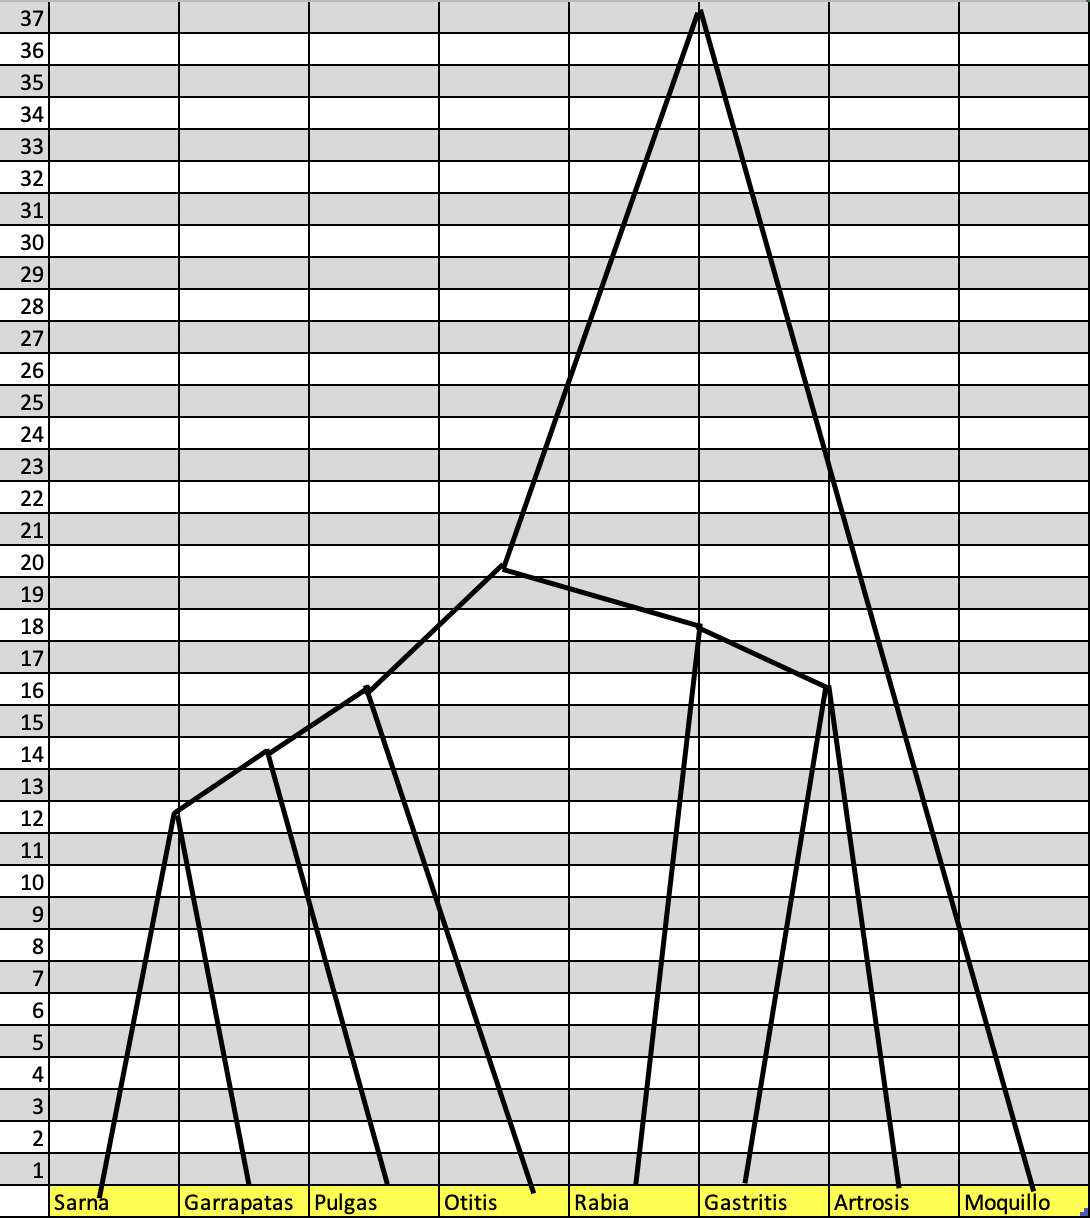
\includegraphics[scale=0.8]{./img/arbol1.png}

\subsection{Árbol de características}
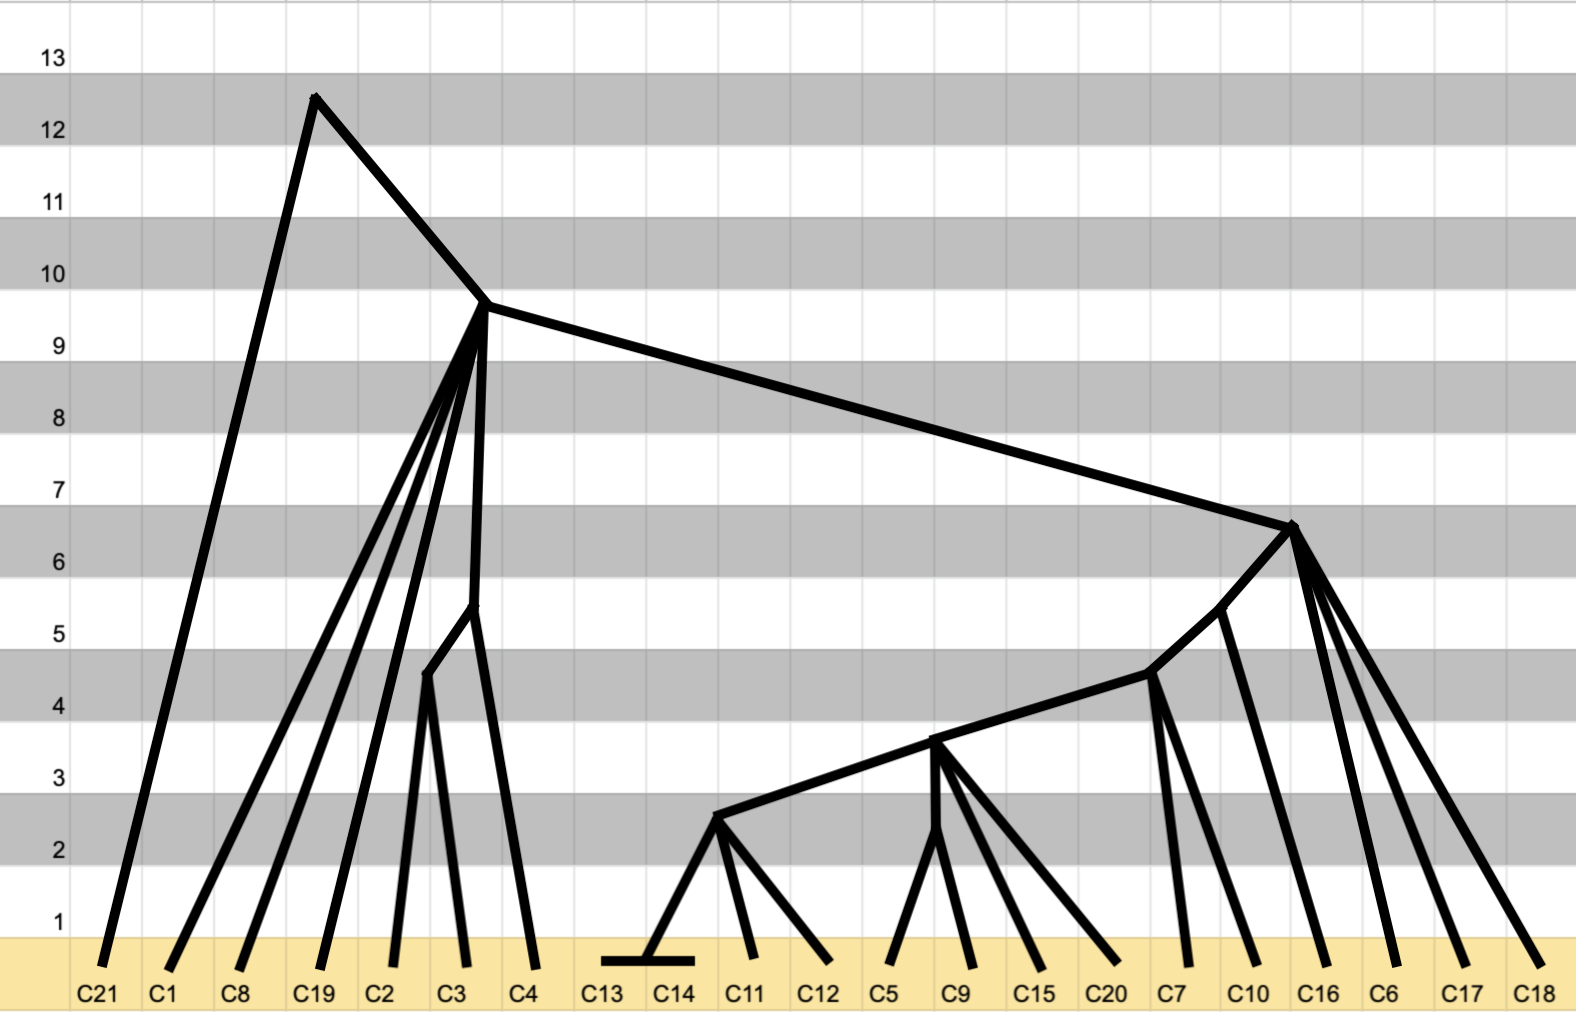
\includegraphics[scale=0.6]{./img/arbol_caracteristicas.png}

\section{Conocimiento estratégico}
\subsection{Árbol de descomposición funcional}
\begin{figure}[H]
\centering
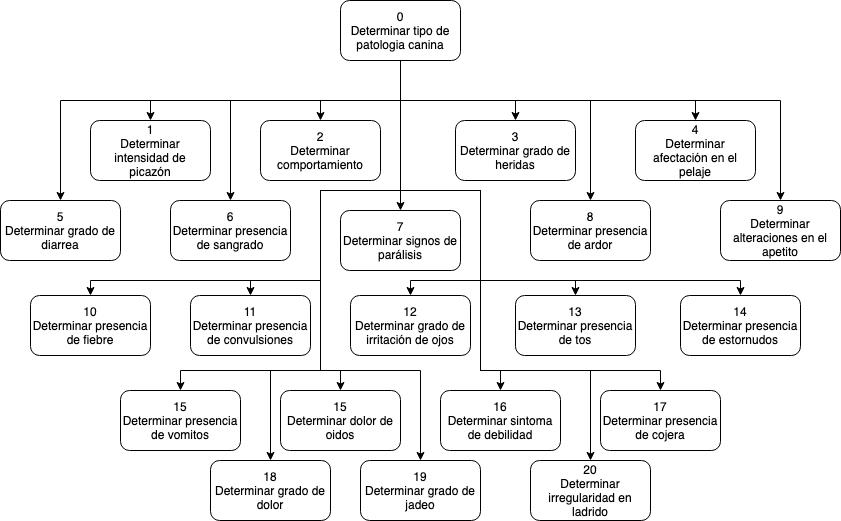
\includegraphics[scale=0.60]{./img/arbol_fallas.png}
\end{figure}

\subsection{Definición de pasos procedurales}

% Please add the following required packages to your document preamble:
% \usepackage{longtable}
% Note: It may be necessary to compile the document several times to get a multi-page table to line up properly
\begin{longtable}{|l|l|}
\hline
\textbf{Nombre de la estrategia} & Determinar intensidad de picazón                                      \\ \hline
\endhead
%
\textbf{Objetivo}                & Determinar en que grado de intensidad el perro siente picazón         \\ \hline
\textbf{Precondiciones}          & Se debe tener acceso visual al animal                                 \\ \hline
\textbf{Entradas}                & Estado actual del animal                                              \\ \hline
\textbf{Razonamiento}            & Observar con qué frecuencia el animal se rasca alguna zona del cuerpo \\ \hline
\textbf{Salida}                  & El perro no se rasca, se rasca poco, mucho o constantemente           \\ \hline
\end{longtable}

% Please add the following required packages to your document preamble:
% \usepackage{longtable}
% Note: It may be necessary to compile the document several times to get a multi-page table to line up properly
\begin{longtable}{|l|l|}
\hline
\textbf{Nombre de la estrategia} & Determinar comportamiento                                                        \\ \hline
\endhead
%
\textbf{Objetivo}                & Determinar alguna alteración en el comportamiento normal del animal              \\ \hline
\textbf{Precondiciones}          & Se debe tener acceso visual al animal                                            \\ \hline
\textbf{Entradas}                & Estado actual del animal                                                         \\ \hline
\textbf{Razonamiento}            & Observar al animal durante un tiempo prudencial, si este está inquieto, se mueve \\ \hline
\textbf{Salida}                  & El perro tiene un comportamiento cansino, normal o hiperactivo                   \\ \hline
\end{longtable}

% Please add the following required packages to your document preamble:
% \usepackage{longtable}
% Note: It may be necessary to compile the document several times to get a multi-page table to line up properly
\begin{longtable}{|l|l|}
\hline
\textbf{Nombre de la estrategia} & Determinar grado de heridas                                                 \\ \hline
\endhead
%
\textbf{Objetivo}                & Determinar si el perro presenta heridas y en que grado                      \\ \hline
\textbf{Precondiciones}          & Se debe tener acceso visual al animal                                       \\ \hline
\textbf{Entradas}                & Estado actual del animal                                                    \\ \hline
\textbf{Razonamiento}            & Inspeccionar el estado general del animal, buscando laceraciones o sangrado \\ \hline
\textbf{Salida}                  & El perro no presenta heridas, tiene costras o heridas sangrantes            \\ \hline
\end{longtable}

% Please add the following required packages to your document preamble:
% \usepackage{longtable}
% Note: It may be necessary to compile the document several times to get a multi-page table to line up properly
\begin{longtable}{|m{100pt}|m{300pt}|}
\hline
\textbf{Nombre de la estrategia} & Determinar afectación en el pelaje                                                                         \\ \hline
\endhead
%
\textbf{Objetivo}                & Determinar la presencia de alguna alteracion en el estado natural del pelaje                               \\ \hline
\textbf{Precondiciones}          & Se debe tener acceso visual al animal y contacto                                                           \\ \hline
\textbf{Entradas}                & Estado actual del animal                                                                                   \\ \hline
\textbf{Razonamiento}            & Inspeccionar el pelaje del animal, hacer analisis al tacto buscando debilidad en el pelo o caida del mismo \\ \hline
\textbf{Salida}                  & El perro tiene el pelaje normal, reseco, con caída o sin pelaje                                            \\ \hline
\end{longtable}

% Please add the following required packages to your document preamble:
% \usepackage{longtable}
% Note: It may be necessary to compile the document several times to get a multi-page table to line up properly
\begin{longtable}{|m{100pt}|m{300pt}|}
\hline
\textbf{Nombre de la estrategia} & Determinar grado de diarrea                                                                   \\ \hline
\endhead
%
\textbf{Objetivo}                & Determinar la consistencia de las heces del animal                                            \\ \hline
\textbf{Precondiciones}          & El dueño debe tomar una muestra de las heces                                                  \\ \hline
\textbf{Entradas}                & Muestra de heces                                                                              \\ \hline
\textbf{Razonamiento}            & Realizar inspección visual de las heces, buscando sangrado y analizando consistencia          \\ \hline
\textbf{Salida}                  & El perro no presenta diarrea, tiene las heces algo liquidas o presenta sangrado en las mismas \\ \hline
\end{longtable}

% Please add the following required packages to your document preamble:
% \usepackage{longtable}
% Note: It may be necessary to compile the document several times to get a multi-page table to line up properly
\begin{longtable}{|m{100pt}|m{300pt}|}
\hline
\textbf{Nombre de la estrategia} & Determinar presencia de sangrado                                                                \\ \hline
\endhead
%
\textbf{Objetivo}                & Determinar si el perro tiene algun sangrado                                                     \\ \hline
\textbf{Precondiciones}          & Se debe tener acceso visual al animal                                                           \\ \hline
\textbf{Entradas}                & Estado actual del animal                                                                        \\ \hline
\textbf{Razonamiento}            & Realizar inspección visual del animal en busqueda de sangre                                     \\ \hline
\textbf{Salida}                  & El perro no presenta sangrado, tiene alguna herida abierta o sangra por orificios continuamente \\ \hline
\end{longtable}

% Please add the following required packages to your document preamble:
% \usepackage{longtable}
% Note: It may be necessary to compile the document several times to get a multi-page table to line up properly
\begin{longtable}{|m{100pt}|m{300pt}|}
\hline
\textbf{Nombre de la estrategia} & Determinar signos de parálisis                                                                           \\ \hline
\endhead
%
\textbf{Objetivo}                & Determinar estado de movilidad del animal                                                                \\ \hline
\textbf{Precondiciones}          & Se debe tener acceso visual al animal                                                                    \\ \hline
\textbf{Entradas}                & Estado actual del animal                                                                                 \\ \hline
\textbf{Razonamiento}            & Observar al animal moverse, si puede hacerlo sin dificultad o presenta algun tipo de problema al hacerlo \\ \hline
\textbf{Salida}                  & El perro camina normalmente, presenta entumecimiento de alguna pata o no puede moverse                   \\ \hline
\end{longtable}

% Please add the following required packages to your document preamble:
% \usepackage{longtable}
% Note: It may be necessary to compile the document several times to get a multi-page table to line up properly
\begin{longtable}{|m{100pt}|m{300pt}|}
\hline
\textbf{Nombre de la estrategia} & Determinar presencia de ardor                                                                   \\ \hline
\endhead
%
\textbf{Objetivo}                & Determinar si el animal siente ardor en alguna zona                                             \\ \hline
\textbf{Precondiciones}          & Se debe tener acceso al animal                                                                  \\ \hline
\textbf{Entradas}                & Estado actual del animal                                                                        \\ \hline
\textbf{Razonamiento}            & Tocar al animal en distintas zonas del cuerpo, buscando zonas enrojecidas o suceptibles         \\ \hline
\textbf{Salida}                  & El perro no presenta ardor, reacciona ante el tacto en cierta zona o enrojecimiento de la misma \\ \hline
\end{longtable}

% Please add the following required packages to your document preamble:
% \usepackage{longtable}
% Note: It may be necessary to compile the document several times to get a multi-page table to line up properly
\begin{longtable}{|m{100pt}|m{300pt}|}
\hline
\textbf{Nombre de la estrategia} & Determinar alteraciones en el apetito                                                                      \\ \hline
\endhead
%
\textbf{Objetivo}                & Determianr si el perro tiene algun tipo de anomalia en el apetito                                          \\ \hline
\textbf{Precondiciones}          & Se debe contar con la presencia del dueño                                                                  \\ \hline
\textbf{Entradas}                & Entrevista con el dueño                                                                                    \\ \hline
\textbf{Razonamiento}            & Consultar al dueño del animal sobre la alimentacion del mismo, si carece de apetito o esta comiendo de mas \\ \hline
\textbf{Salida}                  & El animal presenta falta de apetito, come normalmente o está sobreingiriendo alimento                      \\ \hline
\end{longtable}

% Please add the following required packages to your document preamble:
% \usepackage{longtable}
% Note: It may be necessary to compile the document several times to get a multi-page table to line up properly
\begin{longtable}{|m{100pt}|m{300pt}|}
\hline
\textbf{Nombre de la estrategia} & Determinar presencia de fiebre                                                         \\ \hline
\endhead
%
\textbf{Objetivo}                & Determinar si el perro tiene temperatura                                               \\ \hline
\textbf{Precondiciones}          & Se debe contar con un termometro                                                       \\ \hline
\textbf{Entradas}                & Estado actual del animal                                                               \\ \hline
\textbf{Razonamiento}            & Introducir termometro en el ano del animal, esperar 2 minutos y retirar, ver resultado \\ \hline
\textbf{Salida}                  & El animal no presenta fiebre, tiene fiebre baja, moderada o alta                       \\ \hline
\end{longtable}

% Please add the following required packages to your document preamble:
% \usepackage{longtable}
% Note: It may be necessary to compile the document several times to get a multi-page table to line up properly
\begin{longtable}{|m{100pt}|m{300pt}|}
\hline
\textbf{Nombre de la estrategia} & Determinar presencia de convulsiones                                                                               \\ \hline
\endhead
%
\textbf{Objetivo}                & Determianr si el perro tiene episodios de convulsiones                                                             \\ \hline
\textbf{Precondiciones}          & Se debe contar con la presencia del dueño                                                                          \\ \hline
\textbf{Entradas}                & Entrevista con el dueño                                                                                            \\ \hline
\textbf{Razonamiento}            & Consultar al dueño si ha tenido episodios en el ultimo tiempo. Si el perro actualmente esta convulsionando evaluar \\ \hline
\textbf{Salida}                  & El perro presenta convulsiones esporádicas, no presenta o tiene continuamente                                      \\ \hline
\end{longtable}

% Please add the following required packages to your document preamble:
% \usepackage{longtable}
% Note: It may be necessary to compile the document several times to get a multi-page table to line up properly
\begin{longtable}{|l|l|}
\hline
\textbf{Nombre de la estrategia} & Determinar grado de irritación de ojos                                   \\ \hline
\endhead
%
\textbf{Objetivo}                & Determinar si el perro tiene los ojos irritados por algun malestar       \\ \hline
\textbf{Precondiciones}          & Se debe tener acceso al animal                                           \\ \hline
\textbf{Entradas}                & Estado actual el animal                                                  \\ \hline
\textbf{Razonamiento}            & Inspeccionar ojos del perro, buscando enrojecimiento, lagañas o malestar \\ \hline
\textbf{Salida}                  & El perro presenta ojos normal, resecos, irritados o lagaña permanente    \\ \hline
\end{longtable}

% Please add the following required packages to your document preamble:
% \usepackage{longtable}
% Note: It may be necessary to compile the document several times to get a multi-page table to line up properly
\begin{longtable}{|l|l|}
\hline
\textbf{Nombre de la estrategia} & Determinar presencia de tos                                        \\ \hline
\endhead
%
\textbf{Objetivo}                & Determinar si el perro tiene tos                                   \\ \hline
\textbf{Precondiciones}          & Se debe tener acceso al animal                                     \\ \hline
\textbf{Entradas}                & Estado actual el animal                                            \\ \hline
\textbf{Razonamiento}            & Observar al animal, viendo si presenta expectoraciones esporadicas \\ \hline
\textbf{Salida}                  & El perro presenta tos o no                                         \\ \hline
\end{longtable}

% Please add the following required packages to your document preamble:
% \usepackage{longtable}
% Note: It may be necessary to compile the document several times to get a multi-page table to line up properly
\begin{longtable}{|m{100pt}|m{300pt}|}
\hline
\textbf{Nombre de la estrategia} & Determinar presencia de estornudos                                                                    \\ \hline
\endhead
%
\textbf{Objetivo}                & Determinar si el perro estornuda                                                                      \\ \hline
\textbf{Precondiciones}          & Se debe tener acceso al animal                                                                        \\ \hline
\textbf{Entradas}                & Estado actual el animal                                                                               \\ \hline
\textbf{Razonamiento}            & Observar al animal, viendo si presenta estornudos voluntariamente o ante la presencia de algun objeto \\ \hline
\textbf{Salida}                  & El perro presenta estornudos involuntarios, no presenta o presenta ante la presencia de algun objeto  \\ \hline
\end{longtable}

% Please add the following required packages to your document preamble:
% \usepackage{longtable}
% Note: It may be necessary to compile the document several times to get a multi-page table to line up properly
\begin{longtable}{|m{100pt}|m{300pt}|}
\hline
\textbf{Nombre de la estrategia} & Determinar presencia de vomitos                                                                                    \\ \hline
\endhead
%
\textbf{Objetivo}                & Determinar si el perro regurgita la comida luego de consumir                                                       \\ \hline
\textbf{Precondiciones}          & Se debe tener acceso al dueño                                                                                      \\ \hline
\textbf{Entradas}                & Entrevista con el dueño                                                                                            \\ \hline
\textbf{Razonamiento}            & Consultar al dueño del animal si este ha vomitado en el ultimo tiempo, despues de comer o aun sin ingerir alimento \\ \hline
\textbf{Salida}                  & El perro no presenta vomitos, vomita luego de comer o vomita incluso sin haber ingerido alimento                   \\ \hline
\end{longtable}

% Please add the following required packages to your document preamble:
% \usepackage{longtable}
% Note: It may be necessary to compile the document several times to get a multi-page table to line up properly
\begin{longtable}{|m{100pt}|m{300pt}|}
\hline
\textbf{Nombre de la estrategia} & Determinar dolor de oidos                                                                                             \\ \hline
\endhead
%
\textbf{Objetivo}                & Determinar si el animal presenta algun tipo de dolencia en sus orejas                                                 \\ \hline
\textbf{Precondiciones}          & Se debe tener acceso al animal                                                                                        \\ \hline
\textbf{Entradas}                & Estado actual del animal                                                                                              \\ \hline
\textbf{Razonamiento}            & Inspeccionar las orejas del perro, analizando la temperatura de las mismas, olor de la cavidad y dolencias del animal \\ \hline
\textbf{Salida}                  & El perro no presenta dolor, tiene temperatura en el oido u olor putrefacto en el                                      \\ \hline
\end{longtable}

% Please add the following required packages to your document preamble:
% \usepackage{longtable}
% Note: It may be necessary to compile the document several times to get a multi-page table to line up properly
\begin{longtable}{|m{100pt}|m{300pt}|}
\hline
\textbf{Nombre de la estrategia} & Determinar sintoma de debilidad                                                                       \\ \hline
\endhead
%
\textbf{Objetivo}                & Determinar si el animal presenta algun sintoma de debilidad                                           \\ \hline
\textbf{Precondiciones}          & Se debe tener acceso al animal                                                                        \\ \hline
\textbf{Entradas}                & Estado actual del animal                                                                              \\ \hline
\textbf{Razonamiento}            & Realizar inspeccion del perro, viendo como se comporta y si está largo tiempo en el suelo sin moverse \\ \hline
\textbf{Salida}                  & El perro no presenta sintomas de debilidad o esta debil por largos periodos                           \\ \hline
\end{longtable}

% Please add the following required packages to your document preamble:
% \usepackage{longtable}
% Note: It may be necessary to compile the document several times to get a multi-page table to line up properly
\begin{longtable}{|l|l|}
\hline
\textbf{Nombre de la estrategia} & Determinar presencia de cojera                                         \\ \hline
\endhead
%
\textbf{Objetivo}                & Determinar si el animal presenta alguna dificultad al caminar          \\ \hline
\textbf{Precondiciones}          & Se debe tener acceso al animal                                         \\ \hline
\textbf{Entradas}                & Estado actual del animal                                               \\ \hline
\textbf{Razonamiento}            & Observar al perro moverse, haciendo foco en la movilidad de sus patas  \\ \hline
\textbf{Salida}                  & El perro no presenta cojera, recoge una pata al caminar o las arrastra \\ \hline
\end{longtable}

% Please add the following required packages to your document preamble:
% \usepackage{longtable}
% Note: It may be necessary to compile the document several times to get a multi-page table to line up properly
\begin{longtable}{|l|l|}
\hline
\textbf{Nombre de la estrategia} & Determinar grado de dolor                                                       \\ \hline
\endhead
%
\textbf{Objetivo}                & Determinar si el animal presenta algun sintoma de dolor                         \\ \hline
\textbf{Precondiciones}          & Se debe tener acceso al animal                                                  \\ \hline
\textbf{Entradas}                & Estado actual del animal                                                        \\ \hline
\textbf{Razonamiento}            & Observar al perro, analizando si este se queja o se defiende al tacto por dolor \\ \hline
\textbf{Salida}                  & El perro no muestra sintomas de dolor, presenta dolor constantemente o al tacto \\ \hline
\end{longtable}

% Please add the following required packages to your document preamble:
% \usepackage{longtable}
% Note: It may be necessary to compile the document several times to get a multi-page table to line up properly
\begin{longtable}{|l|l|}
\hline
\textbf{Nombre de la estrategia} & Determinar grado de jadeo                                                   \\ \hline
\endhead
%
\textbf{Objetivo}                & Determinar si el animal presenta alguna alteracion respiratoria             \\ \hline
\textbf{Precondiciones}          & Se debe tener acceso al animal                                              \\ \hline
\textbf{Entradas}                & Estado actual del animal                                                    \\ \hline
\textbf{Razonamiento}            & Observar al animal, buscando evidencia de jadeo constante y ritmo del mismo \\ \hline
\textbf{Salida}                  & El perro no jadea, jadea levemente o tiene un jadeo fuerte constantemente   \\ \hline
\end{longtable}

% Please add the following required packages to your document preamble:
% \usepackage{longtable}
% Note: It may be necessary to compile the document several times to get a multi-page table to line up properly
\begin{longtable}{|m{100pt}|m{300pt}|}
\hline
\textbf{Nombre de la estrategia} & Determinar irregularidad en ladrido                                                         \\ \hline
\endhead
%
\textbf{Objetivo}                & Determinar si el animal presenta alguna alteracion en su frecuencia de ladrido              \\ \hline
\textbf{Precondiciones}          & Se debe tener acceso al animal                                                              \\ \hline
\textbf{Entradas}                & Estado actual del animal                                                                    \\ \hline
\textbf{Razonamiento}            & Escuchar al animal ladrar, prestando atencion a la frecuencia del ladrido, volumen y timbre \\ \hline
\textbf{Salida}                  & El perro no ladra, ladra debilmente o ladra constantemente de forma nerviosa                \\ \hline
\end{longtable}

\section{Conocimiento táctico}
\subsection{Tabla de decisión}
\begin{table}[H]
\centering
\begin{tabular}{|l|l|l|l|}
\hline
\textbf{Condición}       & R1 & R2 & R3 \\ \hline
Picazón & Intensa & Intensa & Intensa   \\ \hline
Comportamiento & Inquieto & Inquieto   & Inquieto    \\ \hline
Heridas & No  &  Si  & No   \\ \hline
Estado de pelaje & Con Insectos & Con insectos   & Normal    \\ \hline
Estado de heces &  Normal  & Normal    & Normal    \\ \hline
Sangrado & No &  Si  & No   \\ \hline
Parálisis & No & Si & No   \\ \hline
Ardor & Si & Si    & Si    \\ \hline
Apetito & Normal & Normal    & Normal    \\ \hline
Fiebre & No & No   & Baja    \\ \hline
Convulsiones & No & No   & No    \\ \hline
Estado de ojos & Normal & Normal   & Normal    \\ \hline
Tos & No & No   & No    \\ \hline
Estornudos & No & No   & No    \\ \hline
Vómito & No & No   & No    \\ \hline
Estado de oídos & Normal & Normal   & Con olor    \\ \hline
Debilidad & No & Si   & No   \\ \hline
Cojera & No & No   & No    \\ \hline
Dolor & No & No   & No   \\ \hline
Jadeo & No & No  & No   \\ \hline
Ladridos & Normal & Normal   & Normal   \\ \hline
\textbf{Acción}          &    &    &    \\ \hline
Tipo de patología canina & Pulgas & Garrapatas & Otitis \\ \hline
\end{tabular}
\end{table}

\begin{table}[H]
\centering
\begin{tabular}{|l|l|l|l|}
\hline
\textbf{Condición}       & R4 & R5 & R6 \\ \hline
Picazón & Intensa  & No   & Normal   \\ \hline
Comportamiento & Decaido & Nervioso   & Nervioso   \\ \hline
Heridas & Si & No   & No   \\ \hline
Estado de pelaje & Con caidas severas  & Normal   & Normal   \\ \hline
Estado de heces & Normal & Normal   & Normal   \\ \hline
Sangrado & Moderado & No   & No   \\ \hline
Parálisis & No & Si    & Si   \\ \hline
Ardor & Si & No   & Si   \\ \hline
Apetito & Leve & Normal    & Normal   \\ \hline
Fiebre & No & Baja   & Alta   \\ \hline
Convulsiones & No & Si   & Si   \\ \hline
Estado de ojos & Normal & Normal   & Con pus    \\ \hline
Tos & No & No   & Si   \\ \hline
Estornudos & No & No   & Si    \\ \hline
Vómito & No & No   & Si    \\ \hline
Estado de oídos & Normal & Normal   & Con temperatura   \\ \hline
Debilidad & Si & No   & Si   \\ \hline
Cojera & No & No   & No    \\ \hline
Dolor & No & Si    & Abdominal   \\ \hline
Jadeo & No & No & Si   \\ \hline
Ladridos & Normal & Normal   & Normal   \\ \hline
\textbf{Acción}          &    &    &    \\ \hline
Tipo de patología canina & Sarna & Rabia & Moquillo \\ \hline
\end{tabular}
\end{table}

\begin{table}[H]
\centering
\begin{tabular}{|l|l|l|l|}
\hline
\textbf{Condición}       & R7 & R8 & R9 \\ \hline
Picazón & No & No   &    \\ \hline
Comportamiento & Apatico & Normal   &    \\ \hline
Heridas & No & No   &    \\ \hline
Estado de pelaje & Normal  & Normal    &    \\ \hline
Estado de heces & Normal  & Normal   &    \\ \hline
Sangrado & Si & No   &    \\ \hline
Parálisis & No & No    &    \\ \hline
Ardor & No & No    &    \\ \hline
Apetito & Leve & Normal    &    \\ \hline
Fiebre & No & No   &    \\ \hline
Convulsiones & No & No   &    \\ \hline
Estado de ojos & Normal & Normal   &    \\ \hline
Tos & No & No   &    \\ \hline
Estornudos & No & No   &    \\ \hline
Vómito & Si & No   &    \\ \hline
Estado de oídos & Normal & Normal   &    \\ \hline
Debilidad & Si  & No   &    \\ \hline
Cojera & Si & Si   &    \\ \hline
Dolor & Abdominal & En las extremidades   &    \\ \hline
Jadeo & No & Si    &    \\ \hline
Ladridos & Normal  & Mas de lo normal   &    \\ \hline
\textbf{Acción}          &    &    &    \\ \hline
Tipo de patología canina & Gastritis & Artrosis &  \\ \hline
\end{tabular}
\end{table}

\subsection{Pseudorreglas}

\begin{table}[H]
\centering
\begin{tabular}{|l|l|}
\hline
\textbf{Nombre de la regla} & Texto de la regla \\ \hline
R1 & SI Picazon = Intensa \\
  & Y Comportamiento = Inquieto \\
  & Y Heridas = No \\
  & Y Estado de pelaje = Con Insectos \\
  & Y Estado de heces = Normal \\
  & Y Sangrado = No \\
  & Y Paralisis = No \\
  & Y Ardor = Si \\
  & Y Apetito = Normal \\
  & Y Fiebre = No \\
  & Y Convulsiones = No \\
  & Y Estado de ojos = Normal \\
  & Y Tos = No \\
  & Y Estornudos = No \\
  & Y Vomito = No \\
  & Y Estado de oidos = Normal \\
  & Y Debilidad = No \\
  & Y Cojera = No \\
  & Y Dolor = No \\
  & Y Jadeo = No \\
  & Y Ladridos = Normal \\
  &   ENTONCES \\
  & Tipo = Pulgas \\ \hline
\end{tabular}
\end{table}

\begin{table}[H]
\centering
\begin{tabular}{|l|l|}
\hline
\textbf{Nombre de la regla} & Texto de la regla \\ \hline
R2 & SI Picazon = Intensa \\
  & Y Comportamiento = Inquieto \\
  & Y Heridas = Si \\
  & Y Estado de pelaje = Con Insectos \\
  & Y Estado de heces = Normal \\
  & Y Sangrado = Si \\
  & Y Paralisis = Si \\
  & Y Ardor = Si \\
  & Y Apetito = Normal \\
  & Y Fiebre = No \\
  & Y Convulsiones = No \\
  & Y Estado de ojos = Normal \\
  & Y Tos = No \\
  & Y Estornudos = No \\
  & Y Vomito = No \\
  & Y Estado de oidos = Normal \\
  & Y Debilidad = Si \\
  & Y Cojera = No \\
  & Y Dolor = No \\
  & Y Jadeo = No \\
  & Y Ladridos = Normal \\
  &   ENTONCES \\
  & Tipo = Garrapatas \\ \hline
\end{tabular}
\end{table}

\begin{table}[H]
\centering
\begin{tabular}{|l|l|}
\hline
\textbf{Nombre de la regla} & Texto de la regla \\ \hline
R3 & SI Picazon = Intensa \\
  & Y Comportamiento = Inquieto \\
  & Y Heridas = No \\
  & Y Estado de pelaje = Normal \\
  & Y Estado de heces = Normal \\
  & Y Sangrado = No \\
  & Y Paralisis = No \\
  & Y Ardor = Si \\
  & Y Apetito = Normal \\
  & Y Fiebre = Baja \\
  & Y Convulsiones = No \\
  & Y Estado de ojos = Normal \\
  & Y Tos = No \\
  & Y Estornudos = No \\
  & Y Vomito = No \\
  & Y Estado de oidos = Con olor \\
  & Y Debilidad = No \\
  & Y Cojera = No \\
  & Y Dolor = No \\
  & Y Jadeo = No \\
  & Y Ladridos = Normal \\
  &   ENTONCES \\
  & Tipo = Otitis \\ \hline
\end{tabular}
\end{table}
  
\begin{table}[H]
\centering
\begin{tabular}{|l|l|}
\hline
\textbf{Nombre de la regla} & Texto de la regla \\ \hline
R4 & SI Picazon = Intensa \\
  & Y Comportamiento = Decaido \\
  & Y Heridas = Si \\
  & Y Estado de pelaje = Con caidas severas \\
  & Y Estado de heces = Normal \\
  & Y Sangrado = Si \\
  & Y Paralisis = No \\
  & Y Ardor = Si \\
  & Y Apetito = Leve \\
  & Y Fiebre = No \\
  & Y Convulsiones = No \\
  & Y Estado de ojos = Normal \\
  & Y Tos = No \\
  & Y Estornudos = No \\
  & Y Vomito = No \\
  & Y Estado de oidos = Normal \\
  & Y Debilidad = Si \\
  & Y Cojera = No \\
  & Y Dolor = No \\
  & Y Jadeo = No \\
  & Y Ladridos = Normal \\
  &   ENTONCES \\
  & Tipo = Sarna \\ \hline
\end{tabular}
\end{table}
  
\begin{table}[H]
\centering
\begin{tabular}{|l|l|}
\hline
\textbf{Nombre de la regla} & Texto de la regla \\ \hline
R5 & SI Picazon = No \\
  & Y Comportamiento = Nervioso \\
  & Y Heridas = No \\
  & Y Estado de pelaje = Normal \\
  & Y Estado de heces = Normal \\
  & Y Sangrado = No \\
  & Y Paralisis = Si \\
  & Y Ardor = No \\
  & Y Apetito = Normal \\
  & Y Fiebre = Baja \\
  & Y Convulsiones = Si \\
  & Y Estado de ojos = Normal \\
  & Y Tos = No \\
  & Y Estornudos = No \\
  & Y Vomito = No \\
  & Y Estado de oidos = Normal \\
  & Y Debilidad = No \\
  & Y Cojera = No \\
  & Y Dolor = En las extremidades \\
  & Y Jadeo = No \\
  & Y Ladridos = Normal \\
  &   ENTONCES \\
  & Tipo = Rabia \\ \hline
\end{tabular}
\end{table}
  
\begin{table}[H]
\centering
\begin{tabular}{|l|l|}
\hline
\textbf{Nombre de la regla} & Texto de la regla \\ \hline
R6 & SI Picazon = Normal \\
  & Y Comportamiento = Nervioso \\
  & Y Heridas = No \\
  & Y Estado de pelaje = Normal \\
  & Y Estado de heces = Normal \\
  & Y Sangrado = No \\
  & Y Paralisis = Si \\
  & Y Ardor = Si \\
  & Y Apetito = Normal \\
  & Y Fiebre = Alta \\
  & Y Convulsiones = Si \\
  & Y Estado de ojos = Con pus \\
  & Y Tos = Si \\
  & Y Estornudos = Si \\
  & Y Vomito = Si \\
  & Y Estado de oidos = Con temperatura \\
  & Y Debilidad = Si \\
  & Y Cojera = No \\
  & Y Dolor = Abdominal \\
  & Y Jadeo = Si \\
  & Y Ladridos = Normal \\
  &   ENTONCES \\
  & Tipo = Moquillo \\ \hline
\end{tabular}
\end{table}
  
\begin{table}[H]
\centering
\begin{tabular}{|l|l|}
\hline
\textbf{Nombre de la regla} & Texto de la regla \\ \hline
R7 & SI Picazon = No \\
  & Y Comportamiento = Apatico \\
  & Y Heridas = No \\
  & Y Estado de pelaje = Normal \\
  & Y Estado de heces = Normal \\
  & Y Sangrado = Si \\
  & Y Paralisis = No \\
  & Y Ardor = No \\
  & Y Apetito = Leve \\
  & Y Fiebre = No \\
  & Y Convulsiones = No \\
  & Y Estado de ojos = Normal \\
  & Y Tos = No \\
  & Y Estornudos = No \\
  & Y Vomito = Si \\
  & Y Estado de oidos = Normal \\
  & Y Debilidad = Si \\
  & Y Cojera = Si \\
  & Y Dolor = Abdominal \\
  & Y Jadeo = No \\
  & Y Ladridos = Normal \\
  &   ENTONCES \\
  & Tipo = Gastritis \\ \hline
\end{tabular}
\end{table}
  
\begin{table}[H]
\centering
\begin{tabular}{|l|l|}
\hline
\textbf{Nombre de la regla} & Texto de la regla \\ \hline
R8 & SI Picazon = No \\
  & Y Comportamiento = Normal \\
  & Y Heridas = No \\
  & Y Estado de pelaje = Normal \\
  & Y Estado de heces = Normal \\
  & Y Sangrado = No \\
  & Y Paralisis = No \\
  & Y Ardor = No \\
  & Y Apetito = Normal \\
  & Y Fiebre = No \\
  & Y Convulsiones = No \\
  & Y Estado de ojos = Normal \\
  & Y Tos = No \\
  & Y Estornudos = No \\
  & Y Vomito = No \\
  & Y Estado de oidos = Normal \\
  & Y Debilidad = No \\
  & Y Cojera = Si \\
  & Y Dolor = En las extremidades \\
  & Y Jadeo = Si \\
  & Y Ladridos = Mas de lo normal \\
  &   ENTONCES \\
  & Tipo = Artrosis \\ \hline
\end{tabular}
\end{table}

\section{Conclusiones}
COMPLETAR

\section{Anexo}

\subsection{Cálculos de distancia de emparrillado}

% Please add the following required packages to your document preamble:
% \usepackage{longtable}
% Note: It may be necessary to compile the document several times to get a multi-page table to line up properly
\begin{longtable}{|l|l|l|l|l|l|l|l|l|}
\hline
           & Pulgas & Garrapatas & Otitis & Sarna & Rabia & Moquillo & Gastritis & Artrosis \\ \hline
\endhead
%
Pulgas     & 0      & 14         & 16     & 14    & 20    & 47       & 26        & 26       \\ \hline
Garrapatas &        & 0          & 30     & 12    & 30    & 49       & 32        & 40       \\ \hline
Otitis     &        &            & 0      & 28    & 22    & 37       & 28        & 28       \\ \hline
Sarna      &        &            &        & 0     & 32    & 53       & 28        & 38       \\ \hline
Rabia      &        &            &        &       & 0     & 41       & 18        & 18       \\ \hline
Moquillo   &        &            &        &       &       & 0        & 47        & 51       \\ \hline
Gastritis  &        &            &        &       &       &          & 0         & 16       \\ \hline
Artrosis   &        &            &        &       &       &          &           & 0        \\ \hline
\end{longtable}

% Please add the following required packages to your document preamble:
% \usepackage{longtable}
% Note: It may be necessary to compile the document several times to get a multi-page table to line up properly
\begin{longtable}{|l|l|l|l|l|l|l|l|}
\hline
                 & Garrapatas-Sarna & Pulgas & Otitis & Rabia & Moquillo & Gastritis & Artrosis \\ \hline
\endhead
%
Garrapatas-Sarna & 0                & 14     & 28     & 30    & 49       & 28        & 38       \\ \hline
Pulgas           &                  & 0      & 16     & 20    & 47       & 26        & 26       \\ \hline
Otitis           &                  &        & 0      & 22    & 37       & 28        & 28       \\ \hline
Rabia            &                  &        &        & 0     & 41       & 18        & 18       \\ \hline
Moquillo         &                  &        &        &       & 0        & 47        & 51       \\ \hline
Gastritis        &                  &        &        &       &          & 0         & 16       \\ \hline
Artrosis         &                  &        &        &       &          &           & 0        \\ \hline
\end{longtable}

% Please add the following required packages to your document preamble:
% \usepackage{longtable}
% Note: It may be necessary to compile the document several times to get a multi-page table to line up properly
\begin{longtable}{|l|l|l|l|l|l|l|}
\hline
                        & Garrapatas-Sarna-Pulgas & Otitis & Rabia & Moquillo & Gastritis & Artrosis \\ \hline
\endhead
%
Garrapatas-Sarna-Pulgas & 0                       & 16     & 20    & 47       & 26        & 26       \\ \hline
Otitis                  &                         & 0      & 22    & 37       & 28        & 28       \\ \hline
Rabia                   &                         &        & 0     & 41       & 18        & 18       \\ \hline
Moquillo                &                         &        &       & 0        & 47        & 51       \\ \hline
Gastritis               &                         &        &       &          & 0         & 16       \\ \hline
Artrosis                &                         &        &       &          &           & 0        \\ \hline
\end{longtable}

% Please add the following required packages to your document preamble:
% \usepackage{longtable}
% Note: It may be necessary to compile the document several times to get a multi-page table to line up properly
\begin{longtable}{|l|l|l|l|l|l|}
\hline
                        & Gastritis-Artrosis & Garrapatas-Sarna-Pulgas & Otitis & Rabia & Moquillo \\ \hline
\endhead
%
Gastritis-Artrosis      & 0                  & 26                      & 28     & 18    & 47       \\ \hline
Garrapatas-Sarna-Pulgas &                    & 0                       & 16     & 20    & 47       \\ \hline
Otitis                  &                    &                         & 0      & 22    & 37       \\ \hline
Rabia                   &                    &                         &        & 0     & 41       \\ \hline
Moquillo                &                    &                         &        &       & 0        \\ \hline
\end{longtable}

% Please add the following required packages to your document preamble:
% \usepackage{longtable}
% Note: It may be necessary to compile the document several times to get a multi-page table to line up properly
\begin{longtable}{|l|l|l|l|l|}
\hline
                               & Garrapatas-Sarna-Pulgas-Otitis & Gastritis-Artrosis & Rabia & Moquillo \\ \hline
\endhead
%
Garrapatas-Sarna-Pulgas-Otitis & 0                              & 26                 & 20    & 37       \\ \hline
Gastritis-Artrosis             &                                & 0                  & 18    & 47       \\ \hline
Rabia                          &                                &                    & 0     & 41       \\ \hline
Moquillo                       &                                &                    &       & 0        \\ \hline
\end{longtable}

% Please add the following required packages to your document preamble:
% \usepackage{longtable}
% Note: It may be necessary to compile the document several times to get a multi-page table to line up properly
\begin{longtable}{|l|l|l|l|}
\hline
                               & Gastritis-Artrosis-Rabia & Garrapatas-Sarna-Pulgas-Otitis & Moquillo \\ \hline
\endhead
%
Gastritis-Artrosis-Rabia       & 0                        & 20                             & 41       \\ \hline
Garrapatas-Sarna-Pulgas-Otitis &                          & 0                              & 37       \\ \hline
Moquillo                       &                          &                                & 0        \\ \hline
\end{longtable}

% Please add the following required packages to your document preamble:
% \usepackage{longtable}
% Note: It may be necessary to compile the document several times to get a multi-page table to line up properly
\begin{longtable}{|m{200pt} | m{200pt} | m{50pt} |}
\hline
                                                        & Gastritis-Artrosis-Rabia-Garrapatas-Sarna-Pulgas-Otitis & Moquillo \\ \hline
\endhead
%
Gastritis-Artrosis-Rabia-Garrapatas-Sarna-Pulgas-Otitis & 0                                                       & 37       \\ \hline
Moquillo                                                &                                                         & 0        \\ \hline
\end{longtable}

% Please add the following required packages to your document preamble:
% \usepackage{longtable}
% Note: It may be necessary to compile the document several times to get a multi-page table to line up properly
\begin{longtable}{|m{150pt}|m{150pt}|}
\hline
                                                                 & Gastritis-Artrosis-Rabia-Garrapatas-Sarna-Pulgas-Otitis-Moquillo \\ \hline
\endhead
%
Gastritis-Artrosis-Rabia-Garrapatas-Sarna-Pulgas-Otitis-Moquillo & 0                                                                \\ \hline
\end{longtable}

\subsection{Cálculos de distancia de caracteristicas para emparrillado}

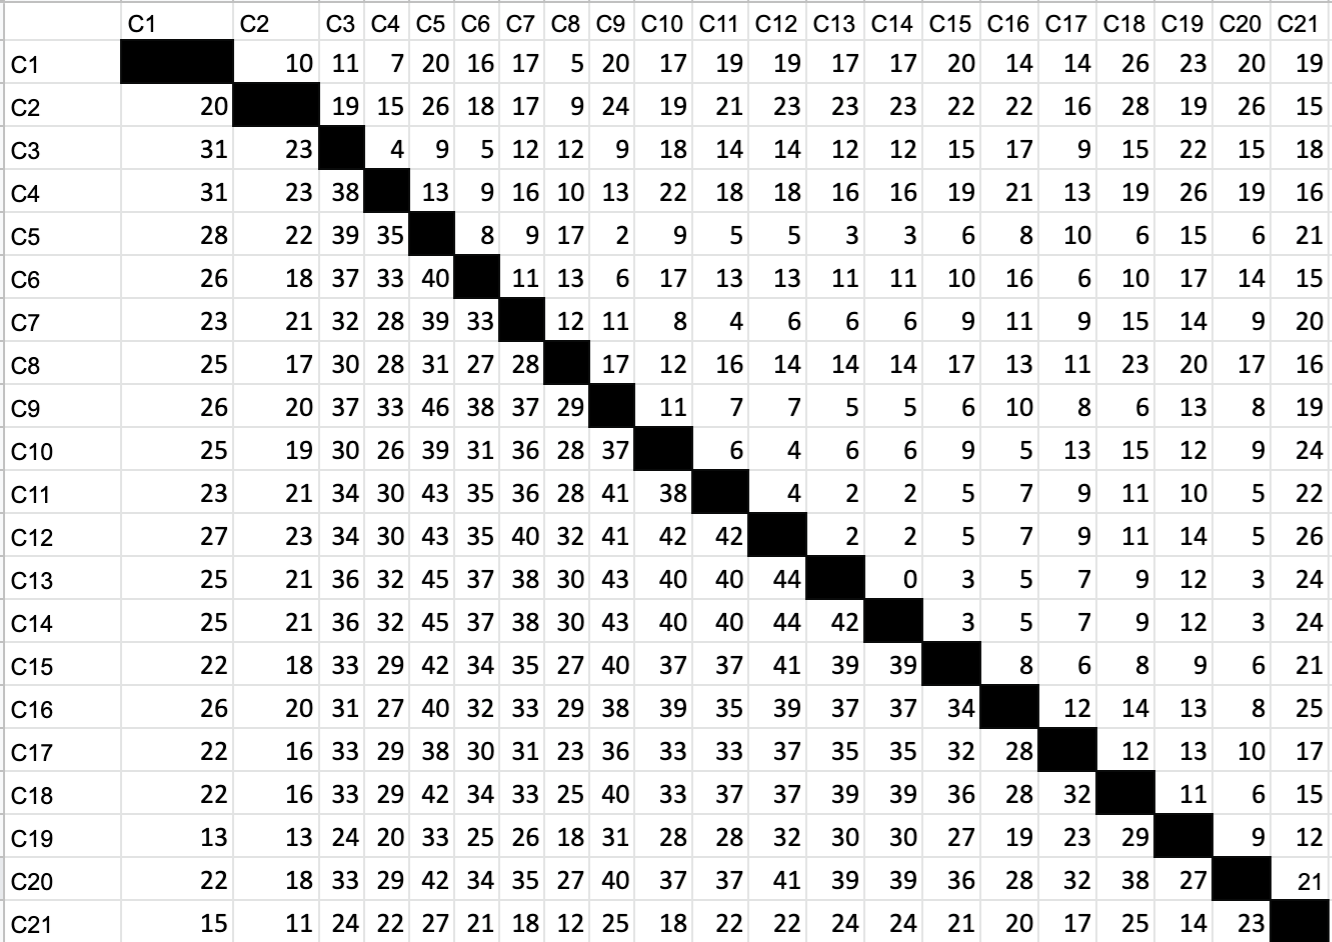
\includegraphics[scale=0.6]{./img/caracteristicas1.png}

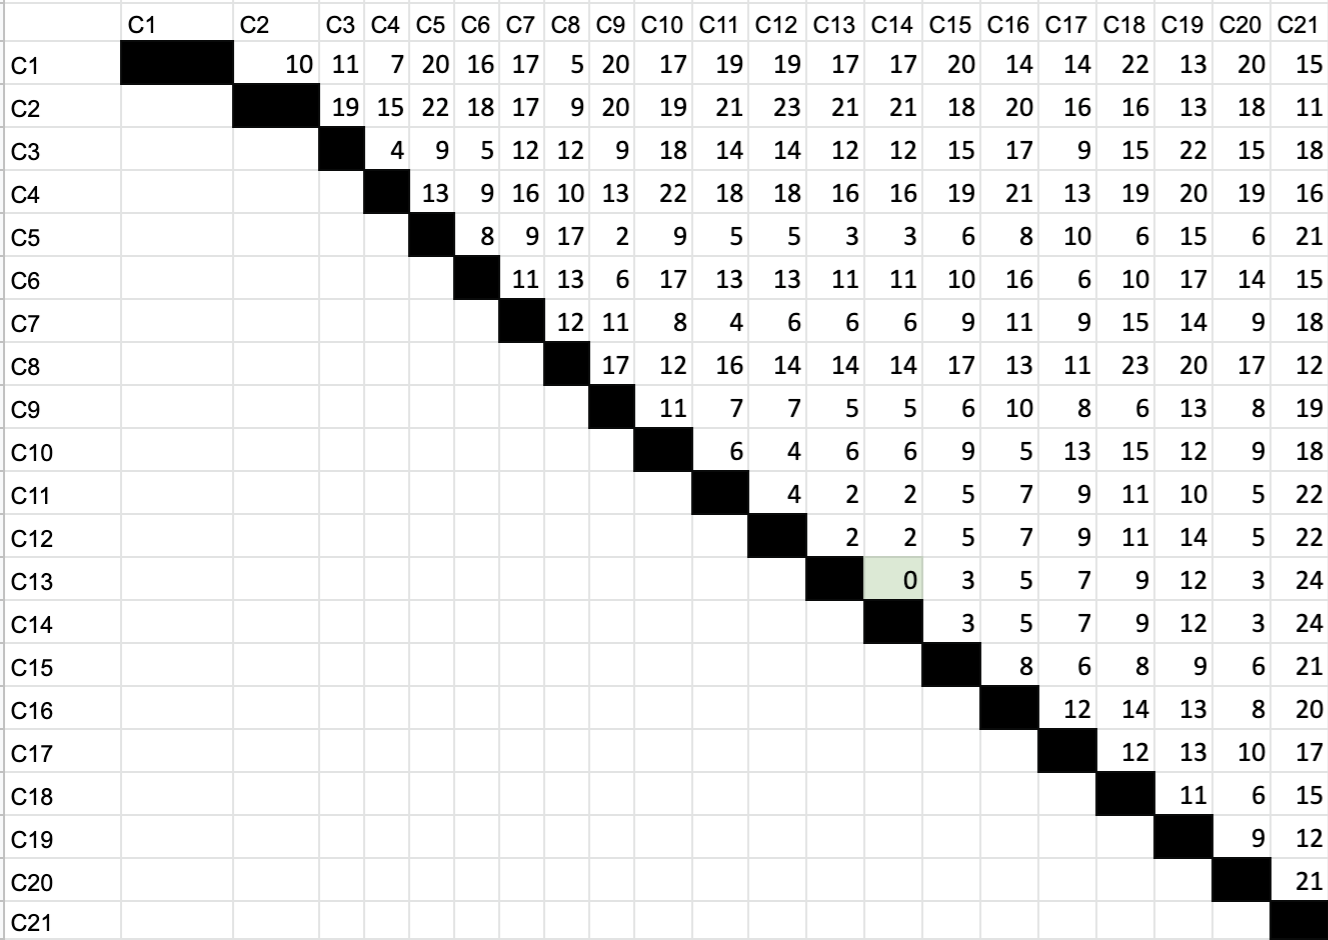
\includegraphics[scale=0.6]{./img/caracteristicas2.png}

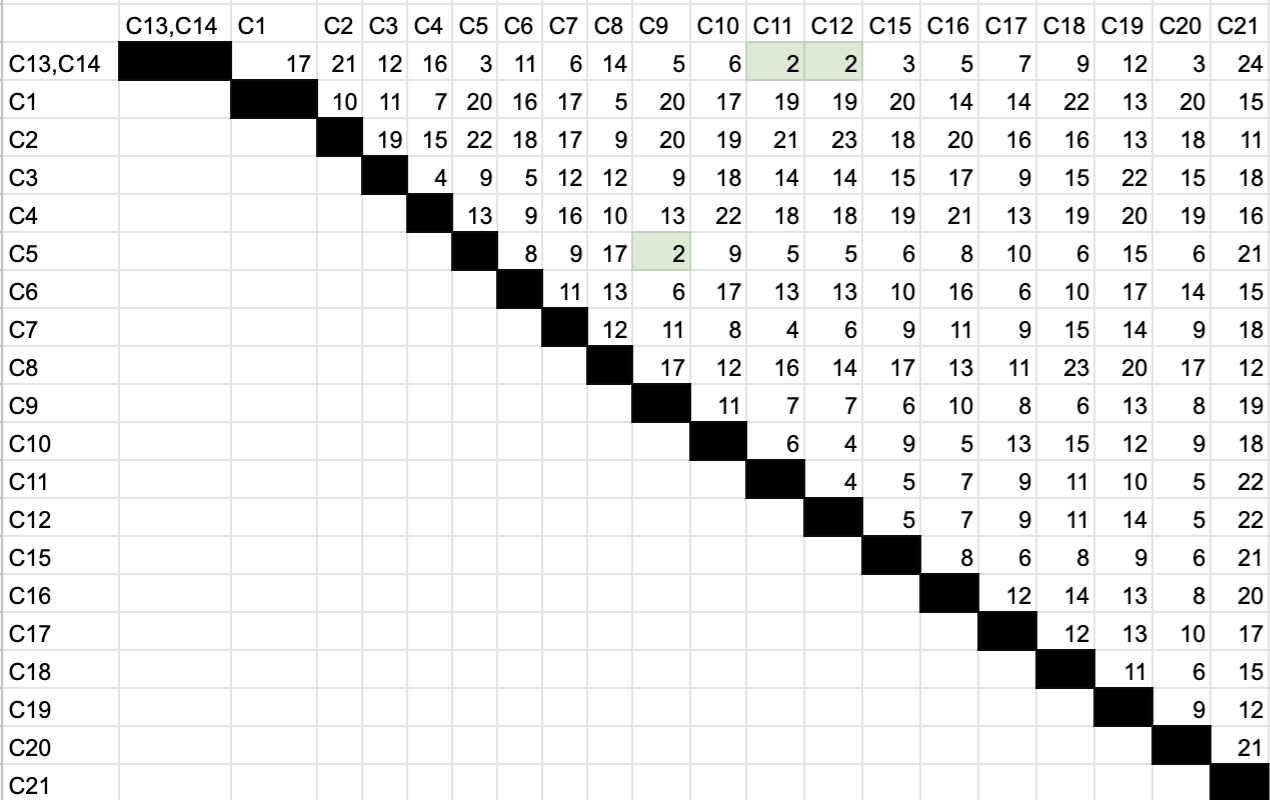
\includegraphics[scale=0.6]{./img/carac3.png}

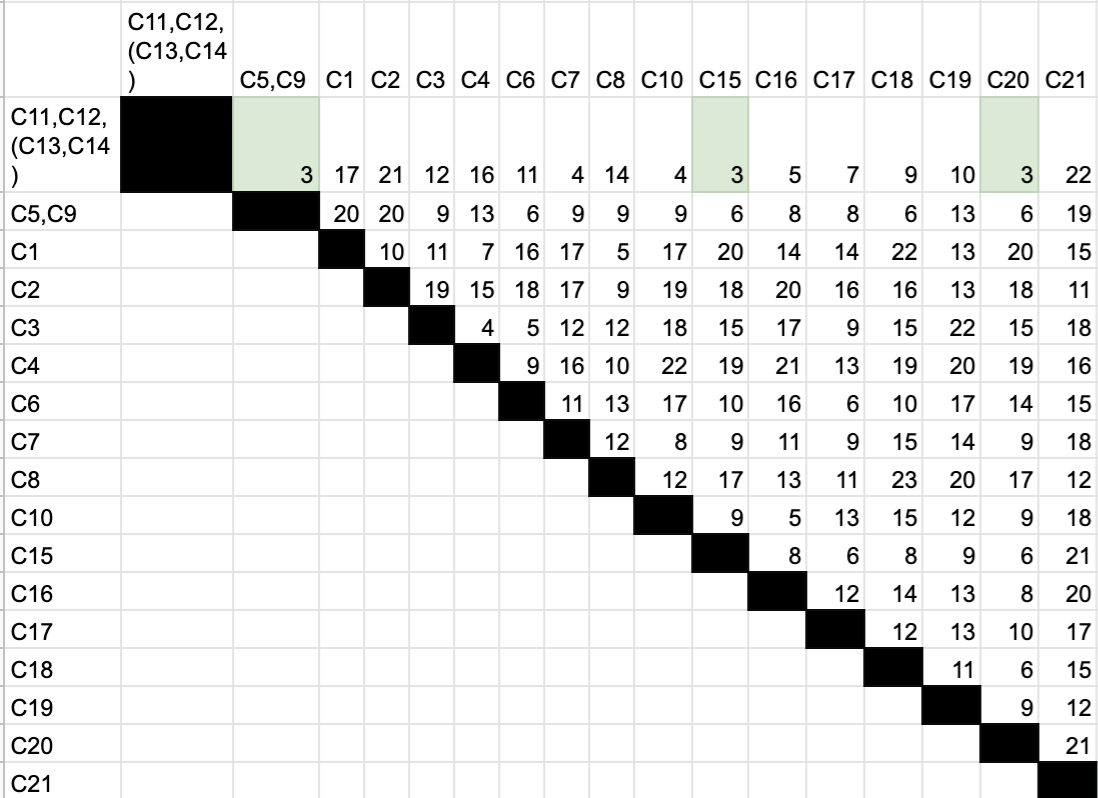
\includegraphics[scale=0.8]{./img/carac4.png}

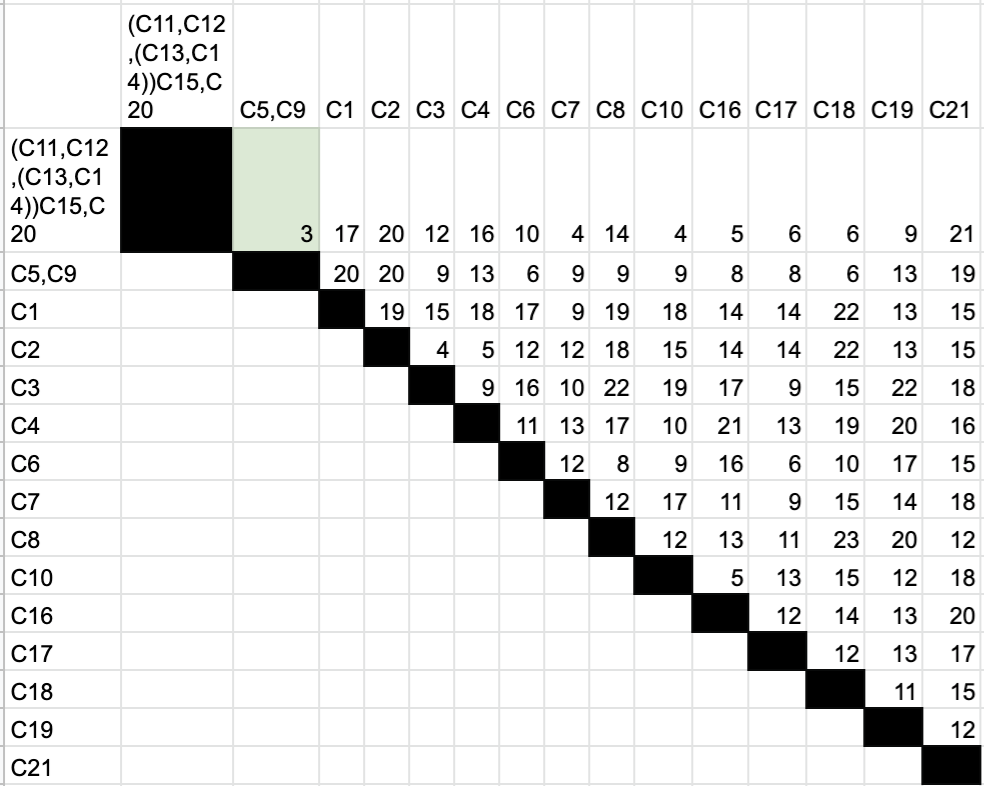
\includegraphics[scale=0.8]{./img/carac5.png}

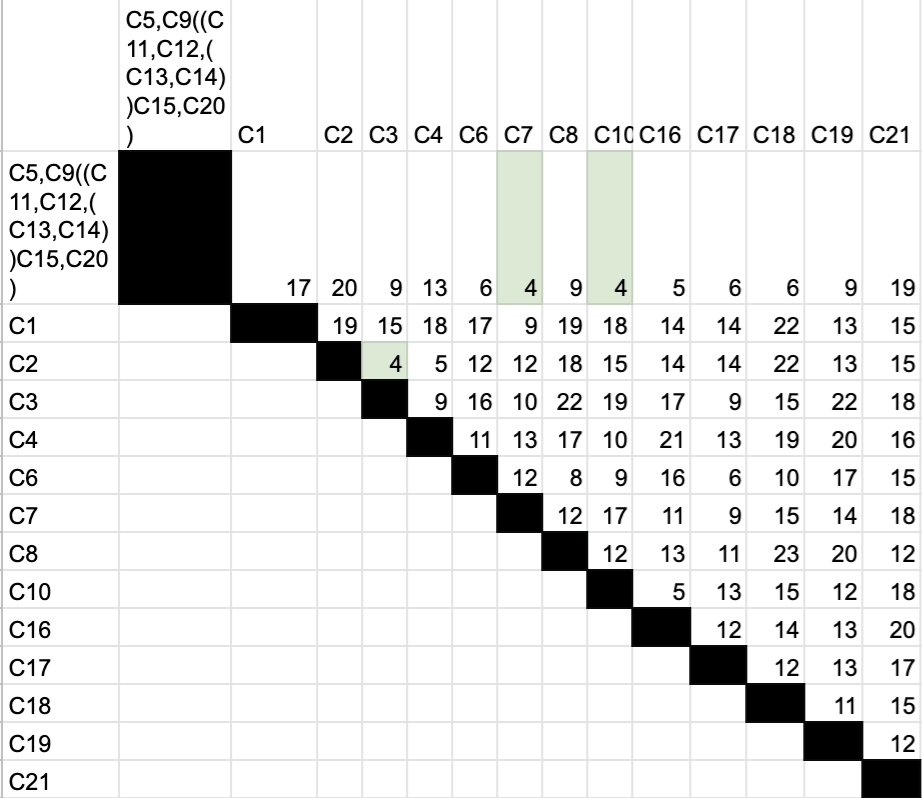
\includegraphics[scale=0.8]{./img/carac6.png}

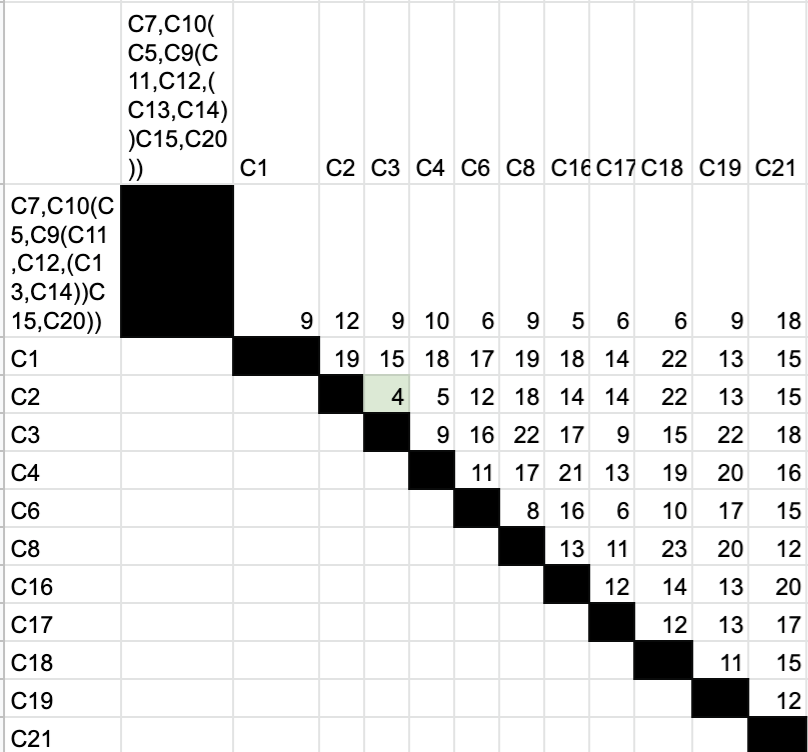
\includegraphics[scale=0.8]{./img/carac7.png}

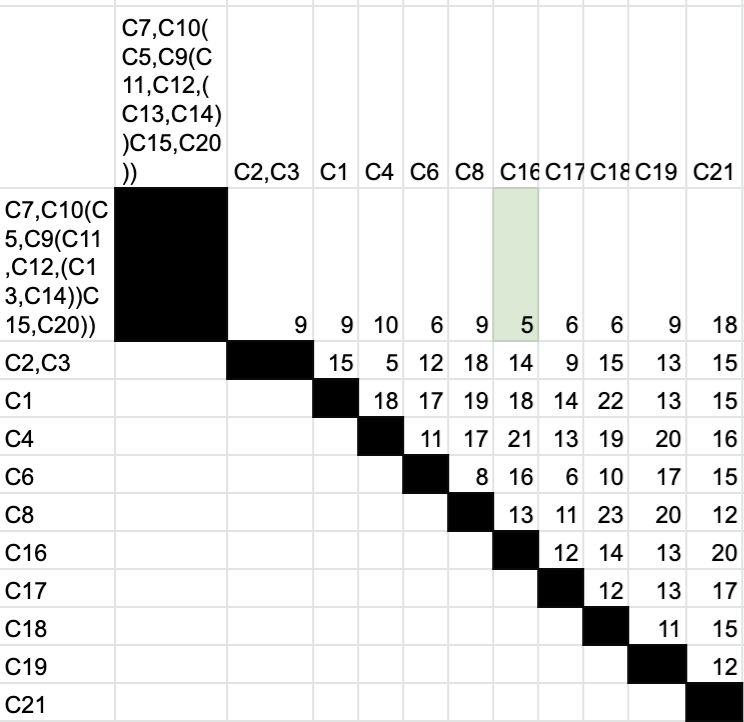
\includegraphics[scale=0.8]{./img/carac8.png}

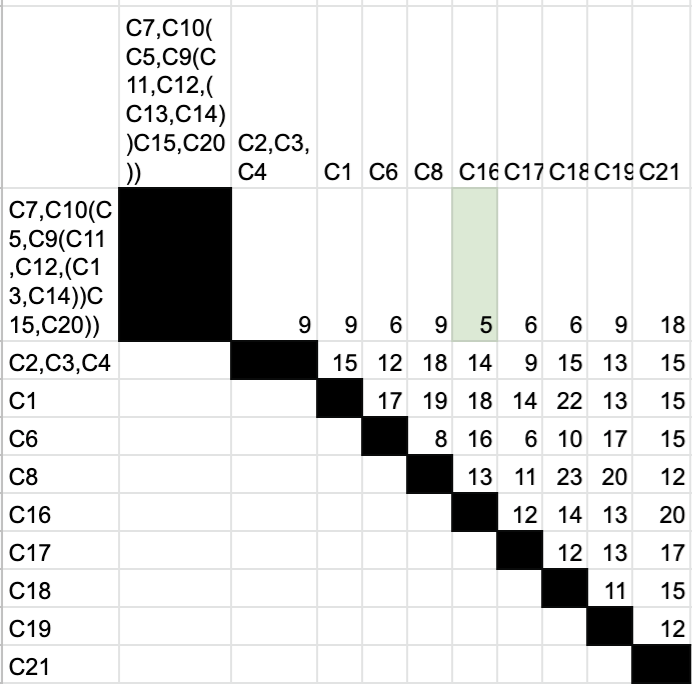
\includegraphics[scale=0.8]{./img/carac9.png}

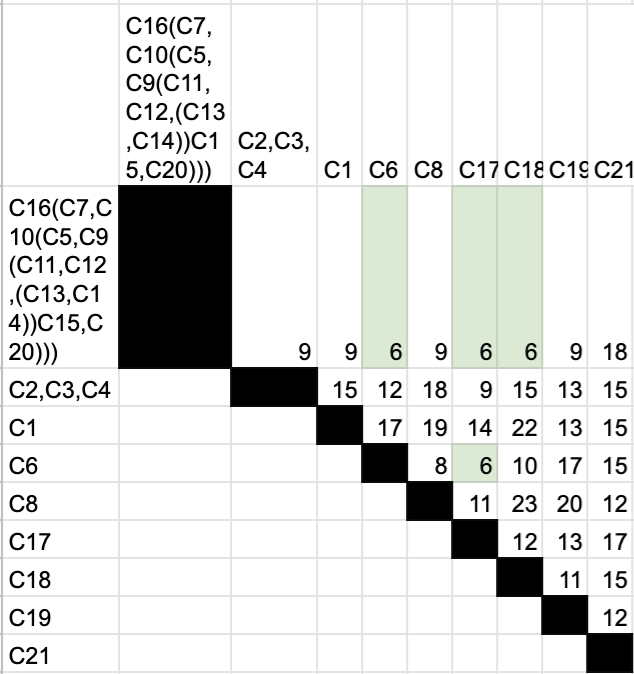
\includegraphics[scale=0.8]{./img/carac10.png}

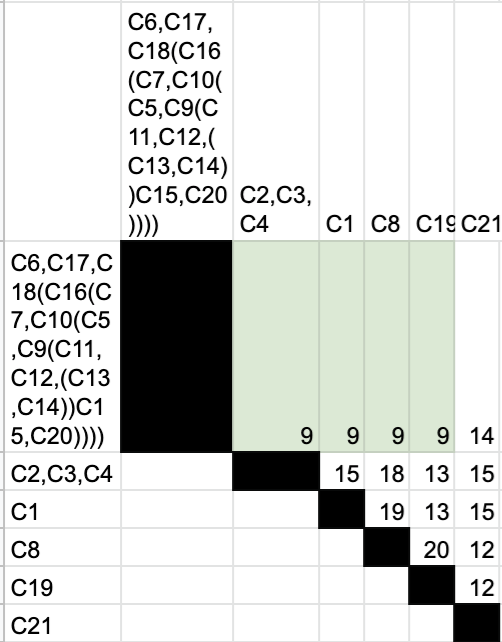
\includegraphics[scale=0.8]{./img/carac11.png}

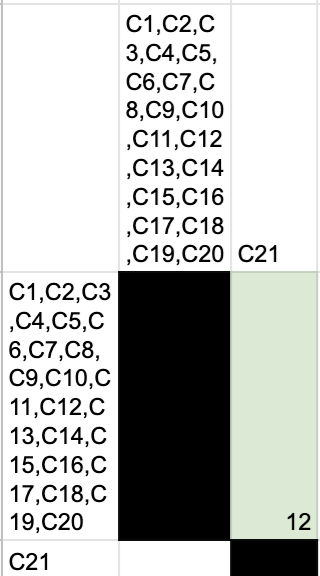
\includegraphics[scale=0.8]{./img/carac12.png}


\end{document}